\documentclass{ximera}


\graphicspath{
  {./}
  {ximeraTutorial/}
  {basicPhilosophy/}
}

\newcommand{\mooculus}{\textsf{\textbf{MOOC}\textnormal{\textsf{ULUS}}}}


\usepackage{tkz-euclide}\usepackage{tikz}
\usepackage{tikz-cd}
\usetikzlibrary{arrows}
\tikzset{>=stealth,commutative diagrams/.cd,
  arrow style=tikz,diagrams={>=stealth}} %% cool arrow head
\tikzset{shorten <>/.style={ shorten >=#1, shorten <=#1 } } %% allows shorter vectors

\usetikzlibrary{backgrounds} %% for boxes around graphs
\usetikzlibrary{shapes,positioning}  %% Clouds and stars
\usetikzlibrary{matrix} %% for matrix
\usepgfplotslibrary{polar} %% for polar plots
\usepgfplotslibrary{fillbetween} %% to shade area between curves in TikZ
\usetkzobj{all}
\usepackage[makeroom]{cancel} %% for strike outs
%\usepackage{mathtools} %% for pretty underbrace % Breaks Ximera
%\usepackage{multicol}
\usepackage{pgffor} %% required for integral for loops



%% http://tex.stackexchange.com/questions/66490/drawing-a-tikz-arc-specifying-the-center
%% Draws beach ball
\tikzset{pics/carc/.style args={#1:#2:#3}{code={\draw[pic actions] (#1:#3) arc(#1:#2:#3);}}}



\usepackage{array}
\setlength{\extrarowheight}{+.1cm}
\newdimen\digitwidth
\settowidth\digitwidth{9}
\def\divrule#1#2{
\noalign{\moveright#1\digitwidth
\vbox{\hrule width#2\digitwidth}}}
























%%This is to help with formatting on future title pages.
\newenvironment{sectionOutcomes}{}{}


\title{Side Lengths}

\begin{document}

\begin{abstract}
Pythagorean Theorem
\end{abstract}
\maketitle




The \textbf{Unit Circle} is the circle on the Cartesian plane of radius $1$ and centered at the origin.


It is the set of points whose distance from the origin is $1$.


We could describe these points with the Complex Number equation $| z | = 1$.



\begin{image}
\begin{tikzpicture}[line cap=round]
  \begin{axis}[
            xmin=-1.1,xmax=1.1,ymin=-1.1,ymax=1.1,
            axis lines=center,
            width=4in,
            xtick={-1,1},
            ytick={-1,1},
            clip=false,
            unit vector ratio*=1 1 1,
            xlabel=$x$, ylabel=$y$,
            ticklabel style={font=\scriptsize},
            every axis y label/.style={at=(current axis.above origin),anchor=south},
            every axis x label/.style={at=(current axis.right of origin),anchor=west},
          ]        
          \addplot [smooth, domain=(0:360)] ({cos(x)},{sin(x)}); %% unit circle

          \addplot [textColor] plot coordinates {(0,0) (.766,.643)}; %% 40 degrees

          \addplot [ultra thick,penColor] plot coordinates {(.766,0) (.766,.643)}; %% 40 degrees
          \addplot [ultra thick,penColor2] plot coordinates {(0,0) (.766,0)}; %% 40 degrees
          
          %\addplot [ultra thick,penColor3] plot coordinates {(1,0) (1,.839)}; %% 40 degrees          

          \addplot [textColor,smooth, domain=(0:40)] ({.15*cos(x)},{.15*sin(x)});
          %\addplot [very thick,penColor] plot coordinates {(0,0) (.766,.643)}; %% sector
          %\addplot [very thick,penColor] plot coordinates {(0,0) (1,0)}; %% sector
          %\addplot [very thick, penColor, smooth, domain=(0:40)] ({cos(x)},{sin(x)}); %% sector
          \node at (axis cs:.15,.07) [anchor=west] {$\theta$};
          \node[penColor, rotate=-90] at (axis cs:.84,.322) {$\sin(\theta)$};
          \node[penColor2] at (axis cs:.383,0) [anchor=north] {$\cos(\theta)$};
          %\node[penColor3, rotate=-90] at (axis cs:1.06,.322) {$\tan(\theta)$};

          \addplot[color=black,fill=black,only marks,mark=*] coordinates{(0.766,0.643)}; 

        \end{axis}
\end{tikzpicture}
\end{image}


We can describe these points with the Cartesian equation $x^2 + y^2 = 1$, the equation for a circle of radius $1$. Also, known as the \textbf{Pythagorean Theorem}.\\



\begin{theorem}   \textbf{\textcolor{green!50!black}{Pythagorean Theorem}} \\

Let $a$ and $b$ be the lengths of the legs of a right triangle. Let $c$ be the length of the hypotenuse. These three numbers satisfy the following equation

\[
a^2 + b^2 = c^2
\]

\end{theorem}




Each point on the Unit Circle sits at the end of a radius and that radius makes an angle with the positive $x$-axis, which is labelled $\theta$ in the diagram.




We have defined the functions sine and cosine as the coordinates of the points on the Unit Circle and the values of these functions depend on the angle $\theta$.

\[    ( \sin(\theta), \cos(\theta) ) \]




And, we know that any right triangle is similar to one of these right triangles defined on the Unit Circle.


This gives us some tools for deducing the lengths of the sides of any right triangle.











\begin{example} 




Determine the length of the side $a$. 






\begin{image}[3in]
    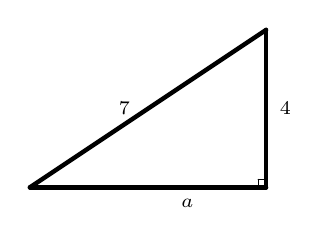
\begin{tikzpicture}[line cap=round]



  \draw [ultra thick] (0,0) -- (3,0);
  \draw [ultra thick] (3,0) -- (3,2);
  \draw [ultra thick] (0,0) -- (3,2);

  \draw [thin] (2.9,0) -- (2.9,0.1);
  \draw [thin] (2.9,0.1) -- (3,0.1);


  %\draw [rotate=0] (0.4,0.13) node {\scriptsize{$\theta$}};


  \draw (3.05,1) node  [anchor=west]{\scriptsize{$4$}};
  \draw (1.2,1) node {\scriptsize{$7$}};
  \draw (2,-0.2) node {\scriptsize{$a$}};





    \end{tikzpicture}
  \end{image}



\begin{explanation}

The sides of a right triangle satisfy the Pythagorean Theorem: $4^2 + a^2 = 7^2$.


\[  16 + a^2 = 49       \]

\[  a^2 = 49 - 16 = \answer{33}     \]

\[  a = \sqrt{33} \, \text{ or } \, a = -\sqrt{33}    \]



Since sides of triangles have a positive length, $a = \sqrt{33}$.



\end{explanation}




\end{example}

















\begin{example}


Determine the length of the side $c$. 






\begin{image}[3in]
    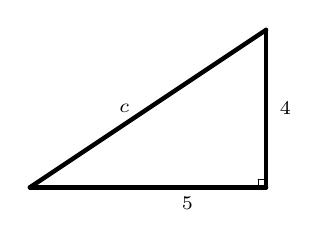
\begin{tikzpicture}[line cap=round]



  \draw [ultra thick] (0,0) -- (3,0);
  \draw [ultra thick] (3,0) -- (3,2);
  \draw [ultra thick] (0,0) -- (3,2);

  \draw [thin] (2.9,0) -- (2.9,0.1);
  \draw [thin] (2.9,0.1) -- (3,0.1);


  %\draw [rotate=0] (0.4,0.13) node {\scriptsize{$\theta$}};


  \draw (3.05,1) node  [anchor=west]{\scriptsize{$4$}};
  \draw (1.2,1) node {\scriptsize{$c$}};
  \draw (2,-0.2) node {\scriptsize{$5$}};





    \end{tikzpicture}
  \end{image}



\begin{explanation}

The sides of a right triangle satisfy the Pythagorean Theorem: $4^2 + 5^2 = c^2$.


\[  16 + 25 = c^2       \]

\[  41 = c^2     \]

\[  c = \sqrt{41} \, \text{ or } \, c = \answer{-\sqrt{41}}    \]



Since sides of triangles have a positive length, $c = \sqrt{41}$.



\end{explanation}




\end{example}






















\section{Algebra}

We have defined the functions sine and cosine as the coordinates of the points on the Unit Circle and the values of these functions depend on the angle $\theta$.

\[    ( \sin(\theta), \cos(\theta) ) \]


These coordinates must satisfy the equation for the Unit Circle. 



\[    ( \sin(\theta) )^2 + ( \cos(\theta) )^2 = 1 \]



From this, we get a list of identities:



\begin{observation}


\begin{itemize}
\item $( \sin(\theta) )^2 + ( \cos(\theta) )^2 = 1$
\item $( \sin(\theta) )^2 =  1 - ( \cos(\theta) )^2$
\item $( \cos(\theta) )^2 =  1 - ( \sin(\theta) )^2$
\item $( \sin(\theta) )^2 =  1 - ( \cos(\theta) )^2 = (1 + \cos(\theta))(1 - \cos(\theta))$
\item $( \cos(\theta) )^2 =  1 - ( \sin(\theta) )^2 = (1 + \sin(\theta))(1 - \sin(\theta))$
\end{itemize}


\end{observation}













\begin{example} Alternate Forms


Transform $\frac{\cos(t)}{1 - \sin(t)}$ into $\frac{1 + \sin(t)}{\cos(t)}$



\begin{explanation}

\begin{align*}
\frac{\cos(t)}{1 - \sin(t)}  &  = &  \frac{\cos(t)}{1 - \sin(t)}  \cdot \frac{1 + \sin(t)}{1 + \sin(t)}  \\
                           &  = &  \frac{\cos(t)(1 + \sin(t))}{(1 - \sin(t))(1 + \sin(t))}  \\
                           &  = &  \frac{\cos(t)(1 + \sin(t))}{1 - (\sin(t))^2}  \\
                           &  = &  \frac{\cos(t)(1 + \sin(t))}{(\cos(t))^2}  \\
                           &  = &  \frac{(1 + \sin(t))}{\cos(t)}  
\end{align*}



\end{explanation}


Well, we have an algebraic alternative.  We have replaced algebraic expressions with equivalent algebraic expressions.  But, we should also think functionally.  That means specifiying domains.  \\


$\blacktriangleright$ As a function, the domain of $\frac{\cos(t)}{1 - \sin(t)}$ does not include and angle where $\sin(t) = 0$. \\

$\blacktriangleright$ As a function, the domain of $\frac{1 + \sin(t)}{\cos(t)}$ does not include and angle where $\cos(t) = 0$. \\



Therefore, $\frac{\cos(t)}{1 - \sin(t)} = \frac{1 + \sin(t)}{\cos(t)}$ for all values except $\left\{   \frac{k \pi}{2} \, | \, k \in \mathbb{Z}      \right\}$

\end{example}










\section{Easy Angles}


From Geometry, we know that an equilateral triangle has equal sides and equal angles.  That makes all of the angles $\frac{\pi}{3}$ radians.  

Let's consider the equilateral triangle below.







\begin{image}
\begin{tikzpicture}[line cap=round]
  \begin{axis}[
            xmin=-1.1,xmax=1.1,ymin=-1.1,ymax=1.1,
            axis lines=center,
            width=4in,
            xtick={-1,1},
            ytick={-1,1},
            clip=false,
            unit vector ratio*=1 1 1,
            xlabel=$x$, ylabel=$y$,
            ticklabel style={font=\scriptsize},
            every axis y label/.style={at=(current axis.above origin),anchor=south},
            every axis x label/.style={at=(current axis.right of origin),anchor=west},
          ]        
          \addplot [smooth, domain=(0:360)] ({cos(x)},{sin(x)}); %% unit circle

          \addplot [textColor] plot coordinates {(0,0) (0.866,0.5)}; %% 30 degrees

          \addplot [ultra thick,penColor] plot coordinates {(0.866,0) (0.866,0.5)}; %% 30 degrees
          \addplot [ultra thick,penColor2] plot coordinates {(0,0) (0.866,0)}; %% 30 degrees
          
          %\addplot [ultra thick,penColor3] plot coordinates {(1,0) (1,.839)}; %% 30 degrees          

          \addplot [textColor,smooth, domain=(0:30)] ({.15*cos(x)},{.15*sin(x)});
          %\addplot [very thick,penColor] plot coordinates {(0,0) (.766,.643)}; %% sector
          %\addplot [very thick,penColor] plot coordinates {(0,0) (1,0)}; %% sector
          %\addplot [very thick, penColor, smooth, domain=(0:40)] ({cos(x)},{sin(x)}); %% sector
          \node at (axis cs:.15,.07) [anchor=west] {$\tfrac{\pi}{6}$};
          \node[penColor, rotate=-90] at (axis cs:.94,.222) {$\sin(\tfrac{\pi}{6})$};
          \node[penColor2] at (axis cs:.5,0) [anchor=north] {$\cos(\tfrac{\pi}{6})$};
          %\node[penColor3, rotate=-90] at (axis cs:1.06,.322) {$\tan(\theta)$};

          \addplot[color=black,fill=black,only marks,mark=*] coordinates{(0.866,0.5)}; 



          \addplot[color=black,fill=black,only marks,mark=*] coordinates{(0.866,-0.5)}; 
          \addplot [ultra thick,penColor] plot coordinates {(0.866,0) (0.866,-0.5)};
          \addplot [textColor] plot coordinates {(0,0) (0.866,-0.5)}; 






        \end{axis}
\end{tikzpicture}
\end{image}






All three sides of the equilateral triangle have equal length and the three angles all measure $\frac{\pi}{3}$.  Since two of the sides are radii of the unti circle, their lengths are $1$.  This makes the length  of the vertical side also $1$.  The vertical side of the triangle is perpendicular to the $x$-axis.  That make the $x$-axis a perpendicular bisector of the equilateral trangle cutting the angle and vertical side into two equal pieces. Each piece of the bisected angle measures $\frac{\pi}{6}$ and the two pieces of the vertical side each of length $\frac{1}{2}$. That tells us that 

\[  \sin\left( \frac{\pi}{6} \right) = \frac{1}{2} \]


The Pythagorean Theorem now tells us that 

\[  1^2 = \left( \sin\left( \frac{\pi}{6} \right) \right)^2 + \left( \cos\left( \frac{\pi}{6} \right) \right)^2  \]


\[  1 = \left( \frac{1}{2} \right)^2 + \left( \cos\left( \frac{\pi}{6} \right) \right)^2  \]


\[  \frac{3}{4} = \left( \cos\left( \frac{\pi}{6} \right) \right)^2  \]



\[  \frac{\sqrt{3}}{2} = \cos\left( \frac{\pi}{6} \right)   \]



And, by similarity:


\[  \cos\left( \frac{\pi}{3} \right) = \frac{1}{2}   \, \text{ and } \,   \sin\left( \frac{\pi}{3} \right)  = \frac{\sqrt{3}}{2} \]  












\begin{center}
\textbf{\textcolor{green!50!black}{ooooo=-=-=-=-=-=-=-=-=-=-=-=-=ooOoo=-=-=-=-=-=-=-=-=-=-=-=-=ooooo}} \\

more examples can be found by following this link\\ \link[More Examples of Right Triangles]{https://ximera.osu.edu/csccmathematics/precalculus2/precalculus2/rightTriangles/examples/exampleList}

\end{center}





\end{document}
